\documentclass[12pt,letterpaper,english,bibliography=totocnumbered, abstract=on]{scrartcl}

\usepackage{indentfirst}
\usepackage[titletoc]{appendix}
%\usepackage{fullpage}
%\usepackage{subfiles}
\usepackage[T1]{fontenc}
\usepackage[latin9]{inputenc}
\usepackage{color}
\usepackage{babel}
\usepackage{verbatim}
\usepackage[unicode=true,pdfusetitle,
bookmarks=true,bookmarksnumbered=false,bookmarksopen=false,
breaklinks=true,pdfborder={0 0 0},pdfborderstyle={},backref=false,colorlinks=true]
{hyperref}
\hypersetup{linkcolor=blue,citecolor=blue,urlcolor=blue}

\usepackage{booktabs}
\usepackage{multirow}
\usepackage{adjustbox}
\usepackage{threeparttable}
\usepackage[table]{xcolor}
\usepackage{csquotes}
\usepackage{soul} % for hiliting text: \hl

\usepackage[backend=biber, style=authoryear, maxbibnames=99, dashed=false]{biblatex}
\setlength\bibitemsep{2\itemsep}
%\addbibresource{mylibrary.bib}
\addbibresource{CRB.bib}

\usepackage{pdfpages}
\usepackage{float} % Allows use of H to place floats

\usepackage{pgfgantt}

\usepackage{framed}

% Prevent page breaks within paragraphs
% https://tex.stackexchange.com/questions/21983/how-to-avoid-page-breaks-inside-paragraphs
\widowpenalties 1 10000

\begin{document}

\titlehead{Grant Proposal: DOI-OIA Coral Reef and Natural Resources Initiative FY2020}

\title{Establishment of Self-sustaining Biological Control of Coconut Rhinoceros Beetle Biotype G in Micronesia }

\author{Aubrey Moore PhD\\University of Guam College of Natural and Applied Sciences}

\maketitle
\newpage
\tableofcontents

\pagebreak

\section{Project Description}

%This grant proposal is a request for funds to hire a post doctoral
%entomologist for 2 years to work on an existing project to implement
%effective biological control for the coconut rhinoceros beetle (CRB)
%which is rapidly killing palm trees in Guam and Palau. Without significant
%population suppression of CRB in Guam and Palau, it is likely that
%Guam and Palau will lose most of their palms and it is just a matter
%of time before other Micronesian Islands are invaded by CRB. 

This grant proposal is a request for funds to support a one-year project with a major goal of establishing effective, self-sustaining biological control of the coconut rhinoceros beetle (CRB) on Guam. \textit{Oryctes rhinoceros}.

\subsection{Background}

\paragraph{The coconut rhinoceros beetle, \emph{Oryctes rhinoceros}, is a major
pest of coconut palm, oil palm and other palm species.}

Palms are damaged when adult beetles bore into the crowns of palms
to feed on sap. Tree mortality occurs when beetles destroy the growing
tip (meristem). Immature beetles (grubs) do no damage. They feed on
dead, decaying vegetation in breeding sites. Preferred breeding sites
are dead, standing coconut stems, and piles of decaying vegetation
such those left behind by typhoons or after replanting of oil palm
plantations. If a CRB population is not suppressed, it is possible
for a positive feed-back cycle to initiate whereby adult beetles kill
massive numbers of palms, thereby generating more food for even more
grubs which turn into adults which kill even more palms. An outbreak
following this scenario occurred in the Palau Islands during the late
1940s resulting in about 50\% coconut palms being killed by CRB throughout
the archipelago and 100\% mortality on some of the smaller islands
(\cite{gressitt_coconut_1953}). A similar outbreak, initiated by Typhoon Dolphin (2015), is currently impacting Guam.

\paragraph{Following 40 years of no geographical range expansion, CRB is again
``on the move'' in the Pacific.}

CRB was recently detected for the first time at several Pacific Island
locations including Saipan (2006), Guam (2007), Port Moresby, Papua
New Guinea (2010), Oahu, Hawaii (2013), Honiara, Solomon Islands
(2015), Rota, CNMI (2017), and Aguiguan, CNMI (2019). 

Eradication of CRB has been attempted many times but is extremely
difficult, having been achieved only once, on Niuatoputapu (formerly
known as Keppel Island), a tiny island belonging to Tonga, with an
area of only 16 km\textsuperscript{2} (3\% the area of Guam) (\cite{catley_coconut_1969}).

Failing eradication, the usual response to CRB infestations during
the second half of the 20th century was introduction of \emph{Oryctes}
nudivirus (OrNV), the biological control agent of choice for this
pest \cite{jackson_use_2009-1} . OrNV attacks only CRB, typically
reducing damage by up to 90\% with population suppression lasting
indefinitely (\cite{bedford_g._o._long-term_2013}). OrNV is auto-disseminated,
meaning the pathogen is carried between feeding and breeding sites
by CRB adults. Like many biocontrol agents, OrNV is density-dependent,
working best at high population densities. After release, OrNV sustains itself within the 
CRB population, limiting damage to very low levels (See Appendix \ref{sub: fiji}: Self-sustaining biological control of CRB in Fiji using OrNV). 

\paragraph*{Current invasions of Pacific Islands by CRB involve a new invasive
biotype that has escaped from biological control by OrNV. }

Discovery of OrNV nudivirus in the 1960s enabled the successful management
of CRB populations in Pacific Island Countries (\cite{huger_oryctes_2005-1}).
Augmentative release of OrNV continues to be an important mechanism
for CRB management in both coconut and oil palm growing regions. For
about 40 years after adoption of this biocontrol strategy,
no new outbreaks of CRB were reported from uninfested palm growing
islands in the Pacific ensuring continuity of palm based village economies. 

However, the situation has recently changed. For the first time in
40 years, CRB invasion into completely new areas has been reported.
Additionally, Pacific areas with established CRB populations (e.g.
Palau) have reported increased severity and frequency of CRB damage.
Common to all these areas is the high incidence of severe palm damage
by beetles not seen since the introduction of OrNV. 

Initial attempts to introduce OrNV into the Guam CRB population were
unexpectedly unsuccessful, raising the possibility that the population
that invaded Guam is tolerant or resistant to the commonly applied
OrNV isolates. Subsequent DNA analysis showed that the Guam population
is genetically different from other populations in the region. On
the basis of distinct genetics and tolerance to currently available
OrNV isolates, the Guam population has been designated a new biotype,
CRB-Guam (CRB-G) (\cite{marshall_new_2015,marshall_new_2017-1}).

DNA analysis from an ongoing survey has detected the CRB-G biotype
in Guam, Hawaii, Palau, Port Moresby (PNG) and Honiara (Solomon Islands).
Thus, current invasions in the Pacific involve the CRB-Guam biotype
and it is expected that these populations are tolerant
isolates of OrNV previously used as biocontrol agents. However, Recent work has identified OrNV isolates which are new biocontrol candidates for CRB-G. (See the \textbf{Recent progress} section below [\ref{recent progress}].)

\paragraph*{Uncontrolled CRB-G outbreaks on islands may kill most palms within a few
years and risk of accidental spread to other islands is high.}

A worse case scenario for a CRB infestation may be triggered by a massive outbreak of adult
CRB emerging from abundant breeding sites made by large amounts of
decaying vegetation left in the wake of a typhoon, from large scale land clearing or large environmental destruction during a war.  The current uncontrolled outbreak on Guam was initiated
by Typhoon Dolphin which visited Guam in May, 2015. Massive amounts of decaying vegetation left in the wake of this storm provided abundant CRB breeding sites. Very high feeding activity by adults emerging 
from these breeding sites killed mature coconut palms, leaving standing dead coconut trunks
which became ideal breeding sites for subsequent generations of beetles. 

During a severe CRB outbreak, there will be an increased risk of further
spread to uninfested islands throughout the Pacific. Palms are important
on Pacific Islands for various reasons: as a cash crop for nuts, oil
and lumber, as an ornamental tree appreciated by residents and tourists.
On some of the smaller, more traditional islands, coconut palm
is referred to as \emph{the tree of life}. On these islands, this species is an
essential natural resource providing income, housing, food, oil, soap,
clothing, mats, baskets, and other containers. The smaller, poorer
Pacific islands will suffer the most if spread of CRB-Guam cannot
be controlled. If CRB-G infests islands and atolls where the coconut
palm as the \emph{tree of life}, islanders may have to migrate to
larger population centers.

\paragraph*{Recommended response to CRB-G invasions.}

Entomologists working on the CRB-G problem agree that the most feasible
way to prevent massive palm mortality during outbreaks is establishment
of biological control using an isolate of OrNV which is highly pathogenic
to CRB-G (\cite{jackson_need_2015,vaqalo_pest_2015,secretariat_of_the_pacific_community_pest_2017}).
%\cite{jackson2015needfor,vaqalo2015anemerging,marshall2016whitepaper}. 

The concensus among Pacific-based entomologists is that the most feasable
way to stop massive palm mortality during CRB-G outbreaks is to find
a find and release a have met several times to plan a response to
CRB-G invasions. In a special meeting on CRB-G at the XXVth International
Congress of Entomology 
%\cite{2016newcoconut}
, the following strategic
plan was suggested:

A coordinated regional project should be organized and adequately
staffed and funded to accomplish 3 objectives:

\begin{enumerate}
	
\item Survey CRB populations throughout the Asian/Pacific region to delimit
the geographical distribution of CRB-G and identify its centre of
origin.

\item Survey CRB-G populations from the centre of origin to find isolate(s)
of OrNV (or other pathogens) that are highly pathogenic for the CRB-G
biotype.

\item Implement \emph{in vivo} or \emph{in vitro} propagation of selected
OrNV isolates for auto-dissemination on islands infested with CRB-G.

\end{enumerate}

The CRB-G problem is not limited to American-affiliated islands. Attempts to find financial support for a well-coordinated Pacific-wide response to this problem have failed. However, there is an \textit{ad hoc} international community of entomologists, the \textit{CRB-G Action Group}, which meets annually (Table \ref{table meetings}).

\begin{table}[H]
	\label{table meetings}
	\centering
	\caption{Meetings of the CRB-G Action Group}
	\begin{tabular}{ll}
		\hline 
		2015 & Pacific Entomology Conference, Honolulu, HI, USA \\ 
		2016 & International Congress of Entomology, Orlando, USA \\
		2017 & Japanese Society for Insect Pathology, Tokyo, Japan \\
		2018 & Society for Invertebrate Pathology, Gold Coast, Australia \\
		2019 & XIX International Plant Protection Congress, Hyderabad, India \\
		2020 & (tentative): Pacific Plant Protection Organization, Guam \\ 
		\hline
\end{tabular}
\end{table}






\paragraph{Recent progress.}
\label{recent progress}

Recent work at the University of Guam, supported by grants from DOI-OIA and USDA-APHIS, has produced encouraging results (See Appendix \ref{section report4}: \textit{DOI-OIA Grant D17AP00107 Progress Report 4} for details):

\begin{itemize}
	
\item	Laboratory tests indicate that OrNV from two sources can be considered as potential biocontrol agents CRB-G: OrNV isolate V23B maintained in insect tissue culture by AgResearch New Zealand and OrNV isolate UOGTW from bodies of CRB collected in Taiwan by the University of Guam CRB-G Biocontrol Project. Further laboratory testing of these virus samples is underway. 
	
\item	PCR tests of recently collected CRB-G adults on Guam indicate presence of OrNV in this population. This virus could be from OrNV autodissemination earlier in the Guam CRB project or from fortuitous introduction.

\end{itemize}
	
%	\textbf{CRB Damage Survey.} A secondary objective of this project is to develop a CRB damage monitoring system. 
%	
%	A digital image analysis system has been developed to detect and quantify V-shaped cuts to fronds and coconut palm mortality caused by CRB. The heart of this system is an object detector, trained by deep learning technology, which locates CRB damage symptoms on frames from georeferenced roadside video surveys. This object detector can be used to automate detection, quantification and to map changes in CRB damage over time and space and can also be used for early detection of CRB invasion.
%	
%	A working prototype of the system has been built.
%	\vspace{0.25in}
%	
%	\textbf{Regional Collaboration.} Uncontrolled outbreaks of CRB-G is a major problem for Pacific islands. Outbreaks of this highly invasive biotype are damaging and killing palms in Guam, Rota, Hawaii, Palau, Papua New Guinea, and the Solomon Islands. Without effective control of these outbreaks, the problem will spread to other Pacific islands, resulting in a human tragedy when it reaches atolls were islanders still rely on coconut palm as the \textit{tree of life}. 
%	
%	Project resources, time and effort were used to facilitate communication among an \textit{ad hoc} collaboration of entomologists working on the CRB-G problem throughout the Pacific. Project staff participated in a symposium and planning meeting of the CRB-G Action Group at the XIX International 
%	Plant Protection Congress in November 2019.
%
%
%
%
%
%
%
%A regional CRB-G biocontrol project has not yet been established because
%funding sources have not been identified.
%
%However, despite relatively scant resources, a USDA-APHIS funded collaboration
%between the University of Guam and AgResearch New Zealand has made
%progress on all 3 objectives:
%\begin{enumerate}
%\item DNA samples from CRB populations collected in Asia indicate the presence
%of the CRB-G biotype in the Philippines and Indonesia.
%\item During a UOG/AgResearch expedition to Negros Island, Philippines in
%January 2017, about 100 DNA samples from a known CRB-G population
%were collected.
%\item Lab tests in at AgResearch New Zealand indicated that all sampled
%beetles belonged to the CRB-G biotype and that one of these was infected
%with OrNV. The OrNV from this beetle was isolated and propagated insect
%cell culture.
%\end{enumerate}
%We are hoping that this OrNV isolate will kill CRB-G adults, to be
%determined in bioassays to be performed on Guam. We are currently
%waiting for APHIS to issue an import permit to allow shipment of a
%sample of the new isolate from New Zealand to Guam. If the isolate
%proves pathogenic for CRB-G, we will immediately start \emph{in vivio}
%propagation and auto-dissemination.

\subsection{Statement of Need}

This proposal is, in part, a response to an urgent need expressed by Micronesian Island leaders in the 22nd Micronesian Islands Forum Communique (Appendix \ref{sec:Extracts-from-the}):

\begin{framed}
In recognition of the urgent need for a Pacific-wide project to find an effective biological control agent for the CRB, the Leaders instructed RISC to seek financial support for such a project, to be conducted with partners at the University of Guam, the Secretariat of the Pacific Community, New Zealand, the USDA and others, as appropriate.
\end{framed}


In addition to loss of coconut as ornamental plants and an emergency food supply, the uncontrolled CRB-G outbreak on Guam is a major environmental disaster rivaling that caused by the brown treesnake (BTS). BTS killed the birds in Guam's forests. CRB-G is now killing the trees. A 2002 US Forest Survey reported that the three most populous trees in Guam's forests were \textit{Cycas micronesica}, \textit{Cocos nucifera} and \textit{Heterospathe elata}  accounting for 16\%, 12\% and 11\% of total trees with a stem diameter of five inches or greater (\cite{moore_failed_2018-1}). These three species, 39\% of the trees in Guam's forests, are being attacked by CRB-G\footnote{Attack of \textit{Cycas micronesica} by CRB-G adults is a recent discovery.}. If the Guam CRB-G outbreak is not brought under control, the island's forest health  will continue to decline, accidental export of CRB-G to other islands in the American Pacific (in addition to Oahu and Rota) will be inevitable and cascading impacts from loss of forests will cause damage to other systems (erosion leading to reef fouling for example).
  
Despite the severity of the Guam CRB-G problem, the US federal government has provided relatively little support for response efforts. USDA-APHIS granted Plant Protection Act funding for CRB-G work in Hawaii and Guam for several years (\cite{moore_usda_2020}). However, a grant proposal requesting \$331,4904 for Guam from FY2020 PPA funding was unexpectedly rejected. A proposal requesting support (\$3.5M) for a cooperative CRB biocontrol project to be performed by North Carolina State University, Colorado State University and the University of Guam has been submitted to DOD's Strategic Environmental Research and Development Program (SERDP). If granted, this SERDP project will begin in the middle of 2021. Thus, \textbf{work towards mitigating the CRB-G problem on Guam during FY2020 is currently unfunded}.

The immediate challenge is to procure bridge funding to retain the Guam Biological Control Project's insect pathologist, Dr. James Grasela, for an additional year so that we can begin propagation and field release of the two OrNV biological control candidates he has identified. Specialized skills of an insect pathologist are essential to implementing successful biological control of CRB-G on Guam and elsewhere.

%This proposal requests funds to hire a post doctoral entomologist
%for 2 years to implement effective biocontrol for CRB. Technical/scientific
%assistance in the form of a post doc is necessary because professional
%capacity to handle major entomological problems in Micronesia is inadequate.
%During the past 2 decades the number of PhD level entomologists practising
%in Micronesia decreased from 9 (5 in Guam, 3 in CNMI, 1 in Palau)
%to 3 (all in Guam). During this same period the workload increased,
%mainly because the detection rate for invasive species went up by
%almost an order of magnitude. The three remaining PhD level entomologists
%in Micronesia do not have time and resources to adequately respond
%to concurrent invasions of coconut rhinoceros beetle, little fire
%ant, Asian cycad scale, and several major agricultural pest insects.
%Teaching and administrative responsibilities do not allow enough time
%to be dedicated to finding solutions to the major entomological problems
%currently impacting Micronesia. The post doctoral entomologist will
%work under supervision of the PI within an existing CRB biocontrol
%program funded by USDA-APHIS. 
%
%Funding of the current proposal will enable extension of benefits
%from the Guam biocontrol project to Palau.
%
%A regional project with the objective of developing effect biological
%control for CRB was identified as an urgent need by Micronesian Governors
%and Presidents at the 22nd Micronesian Islands Forum which took place
%on Guam during May, 2017 (Appendix \ref{sec:Extracts-from-the}).

\subsection{Goals and Objectives}

Recent laboratory bioassays indicate that two recently tested OrNV isolates, V23B and UOGT are potential biocontrol candidates. There is also recent evidence indicating that there is already OrNV actively spreading within the Guam CRB-G population.

\subsubsection{Objective 1: Survey to Determine Background OrNV Incidence} 

CRB adults collected from breeding sites and pheromone traps throughout Guam will by tested for presence of OrNV using PCR.  Laboratory bioassays will be performed on OrNV isolated from these beetles to evaluate potential for biological control. 

\subsubsection{Objective 2: Establish Sustainable CRB-G Biocontrol by Autodissemination of OrNV}

OrNV biocontrol candidates will be propagated \textit{in vivo} using established methods (\cite{huger_oryctes_2005-1}) and released into the Guam CRB-G population by autodissemination. Autodissemination involves infecting healthy CRB adults with OrNV. These infected beetles are then released at points dispersed throughout the island where they vector disease to conspecifics. A permit for field release of OrNV on Guam has already been obtained from USDA-APHIS. Field releases on CEMML on DOD land and by UOG on the rest of Guam. All released beetles will be marked by etching unique numbers on their elytra using a computer-controlled laser engraving system system already in use for this application at UOG.

Beetles for \textit{in vivo} propagation and autodissemination will be field-collected from breeding sites and pheromone traps because this is far more efficient than rearing beetles in the lab at the current time. Impact of virus releases will be monitored using pheromone traps and a novel roadside video analysis system (see Subsection \ref{sub: monitoring}). A subset of beetles captured in traps will be used to estimate the virus infection rate. Concurrent with virus releases, we will continue to screen OrNV isolates to find candidate biocontrol agents.

%We will also perform laboratory bioassays will be performed to quantify the toxic (LD50, LT50, etc.) and nontoxic effects (fecundity, flight capability, etc.) of OrNV on CRB-G. These bioassays will require establishment and maintenance of CRB laboratory colonies. We plan to establish a colony of CRB-G from Guam and also a colony of CRB-S from American Samoa. Availability of these colonies will be used to test two hypotheses:
%
%\begin{description}
%	
%	\item \textbf{Hypothesis 1: CRB-G has a higher tolerance than CRB-S to OrNV isolates previously used for effective biocontrol.} Although CRB-G virus resistance has been presumed, this has not been confirmed by comparative bioassays. 
%	
%	\item \textbf{Hypothesis 2: CRB-G is less attracted than CRB-S to the synthetic aggregation pheromone, oryctalure.} Although CRB pheromone traps baited with oryctalure are widely used, these traps are not very attractive to CRB-G on Guam. When marked beetles were released within grids of pheromone traps, only 8\% of these were recaptured (Moore, unpublished). We will compare responses of CRB-G and CRB-S to oryctalure using a custom-designed y-tube olfactometer \cite{VanderMeer1979} and an electroantennogram. Dr. Michael Orr and his graduate student, Leilani Sablan are planning to do this work.
%	
%\end{description}
%
%Once our lab rearing program is established we will provide CRB-S to collaborators, Dr. Madoka Nakai and Dr. Ross Miller, who are independently investigating the mechanism of virus resistance in CRB-G.

\subsubsection{Objective 3:  Establish Island-wide Monitoring Systems for CRB and Coconut Palm Health}
\label{sub: monitoring}

The CRB-G outbreak on Guam is currently unmonitored on an island-wide basis. An island-wide pheromone trapping system, using about 1500 traps, was operated by the University of Guam from 2008 to 2014. This monitoring system was transferred to the Guam Department of Agriculture which abandoned the effort at the end of February, 2016.  Currently, many coconut palms are being killed by CRB-G. But, in the absence of a monitoring system, we do not have an estimate of tree mortality or whether or not the damage is increasing or decreasing. Clearly, establishment of a monitoring system is necessary to evaluate success of the proposed biocontrol project, or any other mitigation efforts. We intend to re-establish island-wide trapping and to establish a sustainable roadside video survey which uses artificial intelligence to detect CRB damage in dash-cam videos. 

\paragraph{Pheromone Traps}

We plan to installed 150 CRB pheromone monitoring traps. These will be baited with oryctalure and serviced semimonthly. These traps catch approximately equal numbers of males and females which remain alive in the traps for several weeks. Collected beetles will be used for autodissemination of virus and a subsample will be used for virus detection. Traps will be deployed at least 3 months prior to initiation of autodissemination.  

A web database already exists for Guam CRB trap data and it is available for use by this project (URL: \textbf{mysql.guaminsects.net}; database: \textbf{oryctes}; user: \textbf{readonlyguest}; password: \textbf{readonlypassword}; main tables: \textbf{trap} (2,265 records) and \textbf{trap\_visit} (89,114 records)).

\paragraph{Roadside Surveys}

Damage symptoms such as v-shaped cuts to fronds, bore holes, and dead standing coconut palm stems are readily observed during roadside surveys. Survey data will be collected on a smart-phone dash-cam app which georeferences each image. Initially, images of coconut palm damage by CRB-G will be detected, classified and tagged by a technician. When a large number of images have been tagged, these will be used to train an object detector. This work will result in a fully automated CRB damage detection and monitoring system which generates detection alerts and damage maps. This automated system will be useful as an early detection device for CRB. Roadside surveys on Guam will be performed bimonthly and the system will also be tested on Tinian, an island just north of Guam on which CRB has never been detected.

The envisioned system has already been successfully prototyped (See Supporting Technical Data \ref{fig:royal-palms}). A custom object detector for CRB damage has been trained using the TensorFlow implementation of the Faster R-CNN Deep Learning model (Moore, unpublished).








%\subsubsection{Objective 1: Biological Control}
%The major objective is to implement a classical biological control program resulting in establishment of self-sustaining, island-wide control of CRB population on Guam using Oryctes rhinoceros nudivirus (OrNV) as the biological control agent. Based on previous successful CRB biocontrol programs where OrNV was released on other Pacific islands [3, 4], we expect: cessation of mature palm mortality caused by CRB, rapid recovery of damaged palms (Figure 1), and a significantly lower risk of accidental transport of CRB to other islands and beyond. It is expected that this biocontrol will be self-sustaining in Guam as observed elsewhere [5].
%
%\subsubsection{Objective 2: Palm Damage Survey}
%A secondary objective is to establish an island-wide monitoring system to track temporal and spatial changes in the extent of CRB damage to Guam?s coconut palms. Damage symptoms such as V-shaped cuts to fronds, bore holes, and dead standing coconut palm stems are readily observed during roadside surveys. Survey data will be collected using a digital video camera (smart phone) mounted on a truck. Initially, video images of coconut palm damage by CRB-G will be detected, classified and tagged by a technician. When a large number of images have been tagged, these will be used to train an automated CRB damage detection and monitoring system using computer vision and deep learning (Figure 2). This automated system will be useful for monitoring results of biocontrol and other control activities. It may also be used as an early detection device for CRB on neighboring islands at risk of accidental introduction.
%

%The post doctoral entomologist will work on an existing project to
%implement effective biological control for the coconut rhinoceros
%beetle, Guam biotype (CRB-G) which is rapidly killing palm trees in
%Guam and Palau. The overall objective of this project is establish
%a self-sustaining biological control which will stop palm tree mortality
%and eventually suppress the CRB to minimize damage to tolerable levels. 
%
%Details for the following goals can be found in the approved APHIS
%project work plan attached as Appendix \ref{sec:Work-Plan-for}.









%\subsubsection{Perform lab bioassay to determine pathogenicity of the new OrNV isolate
%from Negros Island, Philippines}
%
%If this new isolate is not pathogenic for CRB-G, further foreign eploration
%will be necessary.
%
%\subsubsection{Establish an island-wide coconut palm health survey}
%
%This semiannual health survey will quantify CRB damage to coconut
%palms on an islandwide basis. The survey needs to be started prior
%to auto-dissemination of OrNV or other control tactic is implemented
%so that results can be evaluated.
%
%\subsubsection{Establish a CRB rearing facility to provide adults}
%
%Field collected results will be reared in environmental rearing cabinets
%for use in bioassays, \emph{in vivo} propagation of OrNV and auto-dissemination.
%One rearing cabinet has been ordered. Two more will be ordered with
%FY17 Farm Bill funds.
%
%\subsubsection{Establish biological control of CRB-G by auto-dissemination of OrNV
%in Guam and Palau}
%
%CRB-G adults will be used to autodisemminate OrNV in Guam and Palau.

\subsection{Timeline}

%\begin{figure}[H]
%	%\centering
%	\begin{tikzpicture}
%	\begin{ganttchart}[x unit=0.08in, 
%	y unit chart=0.18in,
%	group label node/.style={text width=2in,align=right,font=\scriptsize\RaggedLeft,anchor=east},
%	bar label node/.style={text width=2in,align=right,font=\scriptsize\RaggedLeft,anchor=east},
%	milestone label node/.style={text width=2in,align=right,font=\scriptsize\RaggedLeft,anchor=east},
%	bar/.append style={fill=lightgray}
%	]{1}{48}
%	
%	\gantttitle{Year}{48} \\
%	\gantttitlelist{1,...,4}{12} \\
%	
%	\ganttgroup{\textbf{Biocontrol}}{1}{48} \\
%	
%	\ganttbar{Continued screening for OrNV biocontrol candidates}{1}{12} \\\\
%	
%	\ganttbar{In vivo virus propagation}{1}{36} \\
%	
%	\ganttbar{OrNV release by autodissemination}{4}{36} \\\\
%	
%	\ganttbar{Sample pheromone trap catch for OrNV}{1}{48} \\\\
%	
%	\ganttbar{Establish of CRB-G and CRB-S lab colonies}{1}{12} \\
%	
%	\ganttbar{Maintain lab colonies}{13}{48} \\\\
%	
%	\ganttbar{Experiments to compare CRB-G and CRB-S}{13}{24} \\\\
%	
%	\ganttmilestone{Decide which OrNV isolate(s) to release}{1} \\
%	
%	\ganttmilestone{Initiate OrNV release}{4} \\\\
%	
%	\ganttmilestone{Review choice of OrNV isolate(s) for release}{13} \\	
%	\ganttmilestone{Annual reports}{13}
%	\ganttmilestone{}{25}
%	\ganttmilestone{}{36}
%	\ganttmilestone{}{48}
%	\\
%	\\
%	
%	\ganttgroup{\textbf{Pheromone trap and video surveys}}{1}{48} \\
%	\ganttbar{Pre-release surveys}{1}{3} \\
%	\ganttbar{Post-release surveys}{4}{48} \\
%	\ganttmilestone{Quarterly survey reports}{4}
%	\ganttmilestone{}{7}
%	\ganttmilestone{}{10}
%	\ganttmilestone{}{13}
%	\ganttmilestone{}{16}
%	\ganttmilestone{}{19}
%	\ganttmilestone{}{22}
%	\ganttmilestone{}{25}
%	\ganttmilestone{}{28}
%	\ganttmilestone{}{31}
%	\ganttmilestone{}{34}
%	\ganttmilestone{}{37}
%	\ganttmilestone{}{40}
%	\ganttmilestone{}{43}
%	\ganttmilestone{}{46} 
%	\\
%	\\
%	
%	\ganttgroup{\textbf{Pacific-wide coordination and collaboration}}{1}{48} 
%	\\
%	
%	\ganttmilestone{Quarterly teleconferences}{3}
%	\ganttmilestone{}{6}
%	\ganttmilestone{}{9}
%	\ganttmilestone{}{12}
%	\ganttmilestone{}{15}
%	\ganttmilestone{}{18}
%	\ganttmilestone{}{21}
%	\ganttmilestone{}{24}
%	\ganttmilestone{}{27}
%	\ganttmilestone{}{30}
%	\ganttmilestone{}{33}
%	\ganttmilestone{}{36}
%	\ganttmilestone{}{39}
%	\ganttmilestone{}{42}
%	\ganttmilestone{}{45}
%	\ganttmilestone{}{48} 
%	\\
%	
%	\ganttmilestone{Annual conferences}{7}
%	\ganttmilestone{}{19}
%	\ganttmilestone{}{31}
%	\ganttmilestone{}{43} 
%	\\
%	\\
%	
%	\ganttgroup{\textbf{SERDP}}{1}{48} 
%	\\
%	
%	\ganttmilestone{Annual progress reports}{14}
%	\ganttmilestone{}{28}
%	\ganttmilestone{}{40} 
%	\\
%	
%	\ganttmilestone{Annual technical meetings}{11} 
%	\ganttmilestone{}{23}
%	\ganttmilestone{}{35}
%	\ganttmilestone{}{47}
%	\\
%	
%	\ganttmilestone{Final report}{48}
%	
%	\ganttlink{elem2}{elem3}
%	\ganttlink{elem5}{elem6}
%	\ganttlink{elem6}{elem7}
%	\ganttlink{elem16}{elem17}
%	
%	\end{ganttchart}	
%	\end{tikzpicture}
%	%\caption{Project schedule.} 
%	%\label{fig:gantt}
%\end{figure}

\begin{ganttchart}[]{1}{12}
	\gantttitle{Month}{12} \\
	\gantttitlelist{1,...,12}{1} \\
	\ganttgroup{Biological Control}{1}{12} \\
%	\ganttbar{Task 1}{1}{2} \\
%	\ganttlinkedbar{Task 2}{3}{7} 
%	\ganttnewline
%	\ganttmilestone{Milestone}{7} \\
%	\ganttnewline
%	\ganttbar{Final Task}{8}{12} \\
%	\ganttlink{elem2}{elem3}
%	\ganttlink{elem3}{elem4}
	
	\ganttbar{Prerelease OrNV survey}{1}{2}\\
	\ganttbar{\textit{In vitro} OrNV propagation}{3}{11}\\
	
	\ganttbar{Autodissemination of OrNV}{3}{11}\\
	
	\ganttgroup{Pheromone traps}{1}{12} \\
	\ganttbar{Deploy traps}{1}{1}\\
	\ganttbar{Check/maintain traps (biweekly)}{2}{12}\\
	
	
	\ganttgroup{Roadside video surveys of CRB damage}{1}{12} \\
	\ganttmilestone{Roadside surveys (bimonthly)}{1}
	\ganttmilestone{}{3}
	\ganttmilestone{}{5}
	\ganttmilestone{}{7}
	\ganttmilestone{}{9}
	\ganttmilestone{}{11} \\
	\ganttbar{Object detector training}{1}{3}\\
	\ganttbar{Automated video analysis}{4}{12}\\
	
		
	\ganttgroup{Reporting}{1}{12} \\
	\ganttmilestone{Trapping and damage survey reports and maps}{2}
	\ganttmilestone{}{4}
	\ganttmilestone{}{6}
	\ganttmilestone{}{8}
	\ganttmilestone{}{10}
	\ganttmilestone{}{12} \\
						
	\ganttmilestone{Semiannual report}{7} \\
	\ganttmilestone{Final report}{12}
\end{ganttchart}

%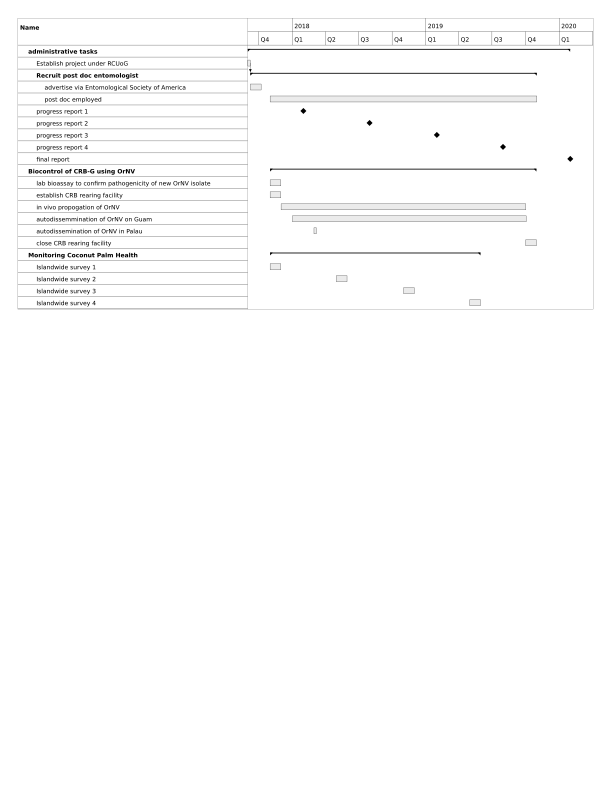
\includegraphics[width=1\textwidth,height=1\textheight,keepaspectratio]{output}.
\newpage
\subsection{Potential Benefits}
\begin{itemize}
\item This project will directly benefit Guam.
Without implementation
of effective biological control, it is likely that 50\% or more coconut
palms will be killed by CRB-G. In addition to loss of coconut as ornamental plants and an emergency food supply, the uncontrolled CRB-G outbreak on Guam is a major environmental disaster with 39\% the trees in Guam's forests are at risk of attack by CRB-G. If the outbreak is not brought under control, the island's forest health  will continue to decline, accidental export of CRB-G to other islands in the American Pacific (in addition to Oahu and Rota) will be inevitable and cascading impacts from loss of forests will cause damage to other systems (erosion leading to reef fouling for example).

\item This project will indirectly benefit all other islands in Micronesia and other areas of the Pacific.
With very high populations of CRB-G in Gaum
risk of accidental introduction to other islands is extremely high.
CRB-G has already been intercepted twice on Saipan, it is established on Rota and it has been detected on Aguiguan. If CRB-G infests smaller islands and atolls in the FSM and RMI
where the coconut palm as the \emph{tree of life}, islanders may have
to migrate to larger population centers. If funded, the proposed project will be run under the \textit{Open Science} concept. All data and analyses will be publicly shared on the internet in near-real time and samples of biocontrol candidates will be also be shared other Pacific islands battling CRB-G. 

\item It is expected that establishment of OrNV as an effective biological control agent will provide permanent self-sustaining population suppression of CRB-G. This is in contrast to temporary results from invasive species control programs which rely on population suppression using pesticide application, trapping or physical removal.

\item Technology developed for automated roadside video surveys may be used for early detection of CRB on islands on which this pest has not yet been detected. Roadside videos may be of use for monitoring spread of invasive weeds such as Mexican creeper, \textit{Antigonon leptopus\textit}.

\end{itemize}

\newpage
\section{Budget}

\begin{center}
\begin{tabular}{lr}
\hline 
\textbf{Item}      & \textbf{Cost}\\
\hline 
Personnel          & \$146,200 \\
Benefits           &  \$43,200 \\
Travel             &   \$4,000 \\
Supplies           &  \$15,290 \\
\hline 
\textbf{SUBTOTAL}  & \textbf{\$208,690} \tabularnewline
\hline
Administrative fee & \$31,304 \tabularnewline
\hline 
\textbf{TOTAL}	   & \textbf{\$239,994} \tabularnewline
\hline 
\end{tabular} 
\par\end{center}

\begin{description}
	
\item [{Personnel}] includes salary for an insect pathologist (Dr. James Grasela, 1 FTE, \$64,000), 
a laboratory technician (Mr. Chris Cayanan, 1 FTE, \$40,000) and a field technician (vacant, 0.9 FTE, \$40,000). Benefits for these 3 positions are calculated at 30\% * salary. Also includes PI's salary compensation calculated at 0.02 FTE * \$110,000.

\item [{Travel}] includes airfare and other relocation expenses for Dr. Grasela who resides in Missouri.

\item [{Supplies}] includes laboratory and insect rearing supplies (\$5,340) and fuel and maintenance for the project's field vehicle (\$4,000), purchase of 100 pheromone traps (\$4,000), and purchase of 520 pheromone lures (\$1,950). 

\item [{Administrative~fee}] equal to 15\% of the total grant award
is charged by the Research Corporation of the University of Guam for
services provided.

\end{description}

\newpage
\printbibliography

\newpage{}

%\bibliographystyle{IEEEtran}
%\phantomsection\addcontentsline{toc}{section}{\refname}\bibliography{references}

\newpage{}
\begin{appendices}

\section{Supporting Technical Data}

\subsection{Self-sustaining Biological Control of CRB in Fiji Using OrNV}
\label{sub: fiji}

\begin{figure}[h]
\centering
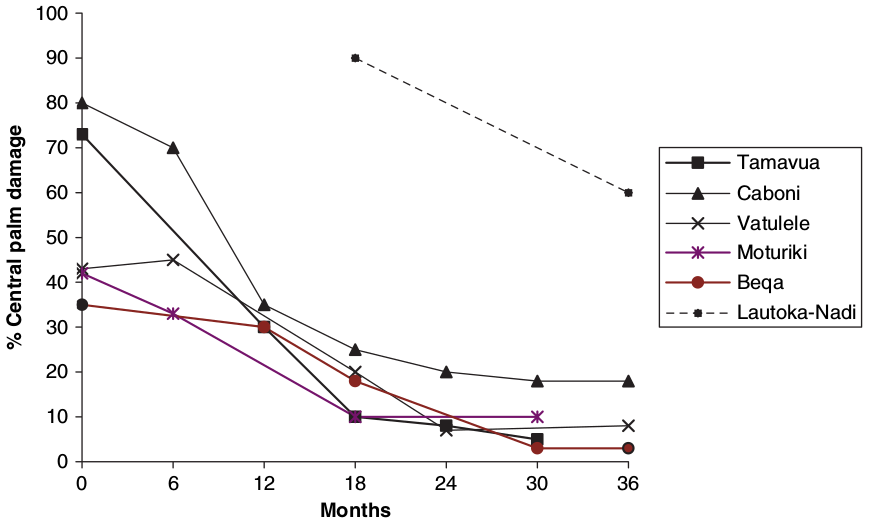
\includegraphics[width=0.7\linewidth]{images/fiji}
\caption{Reduction in coconut palm damage following release of \textit{Oryctes rhinoceros} nudivirus in Fuji. (\cite{jackson_use_2009-1})}
\label{fig:fiji}
\end{figure}

Reduction in palm damage recorded over 36 months after release of \textit{Oryctes virus} on five sites in the Fiji Islands from 1970 to 1972. No virus was released in the Lautoka area where damage remained high 18 months after the start of the program but natural incidence of disease was recorded in the area after 36 months coinciding with a decline in visible damage. Population suppression of CRB by OrNV in Fiji was still in effect 35 years after virus introduction (\cite{bedford_g._o._long-term_2013}).

\clearpage

\subsection{Automated Monitoring of CRB Damage Using Roadside Video Surveys}

\begin{figure}[h]
\centering
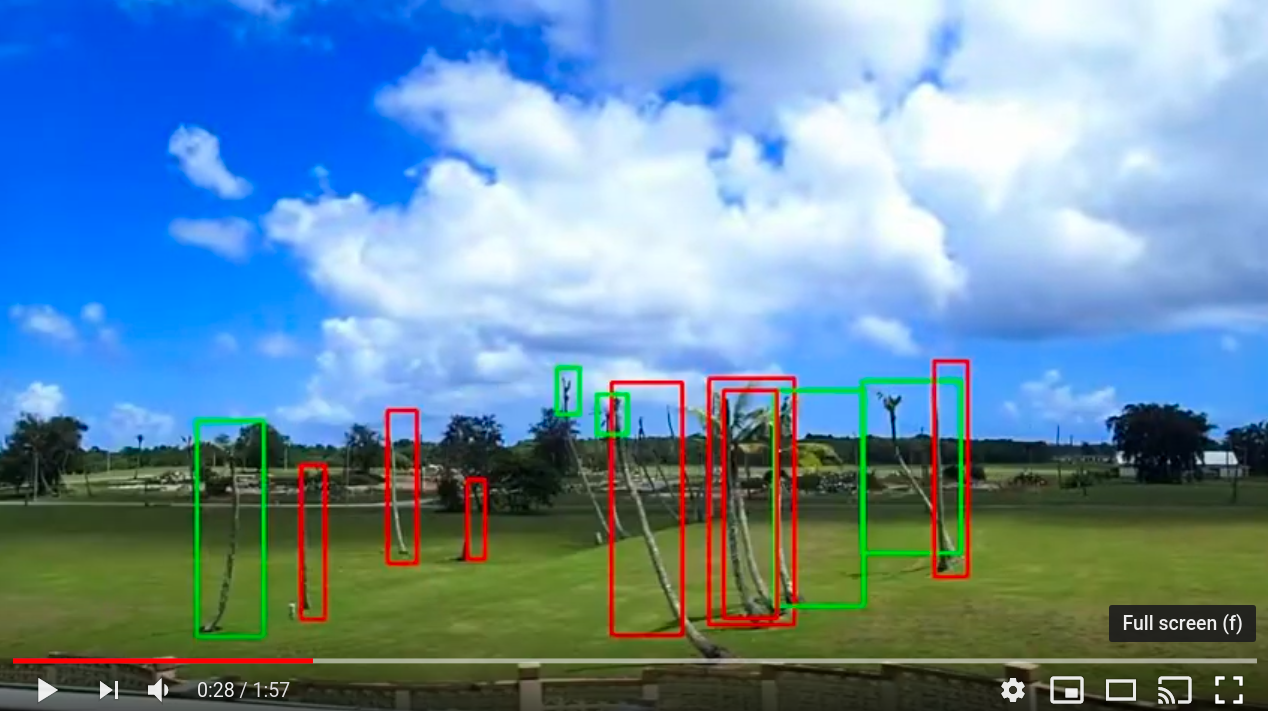
\includegraphics[width=0.7\linewidth]{images/royal-palms}
\caption{Training an Object Detector to Locate Coconut Palms Damaged or Killed by Coconut Rhinoceros Beetle. \url{https://youtu.be/zzSorqcmt9U}.}
\label{fig:royal-palms}
\end{figure}

Result of a first attempt to train an object detector (Faster R-CNN) to locate coconut trees killed or damaged by coconut rhinoceros beetle in a video. Dead palms are in red boxes, damaged palms are in green boxes. Not perfect, but it does serve as a proof of concept.

\clearpage

%\section{USDA-APHIS 2020 Plant Protection Act Proposal (UNFUNDED)}
%Please see next page.
%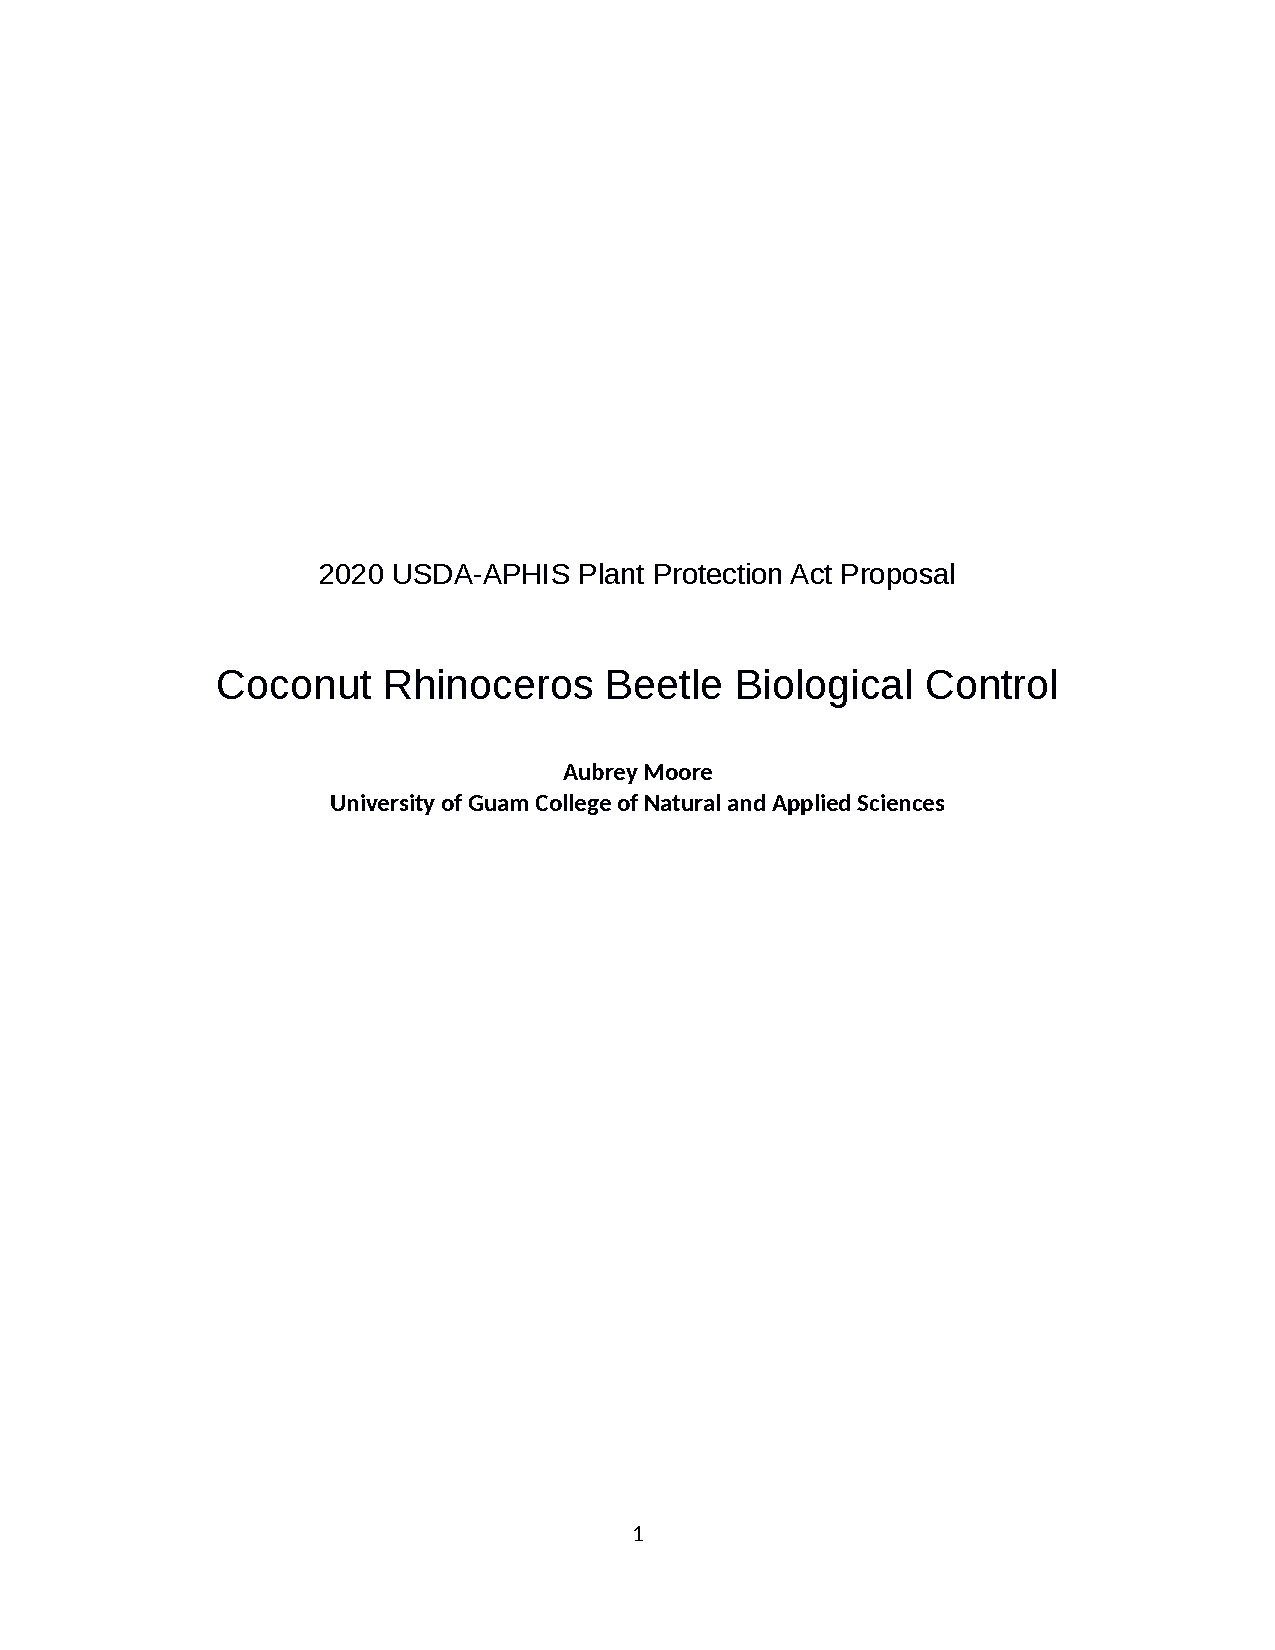
\includepdf[pages=-]{2020-PPA/Moore-FY20-PPA}

\section{DOI-OIA Grant D17AP00107 Progress Report 4}
\label{section report4}
Please see next page.
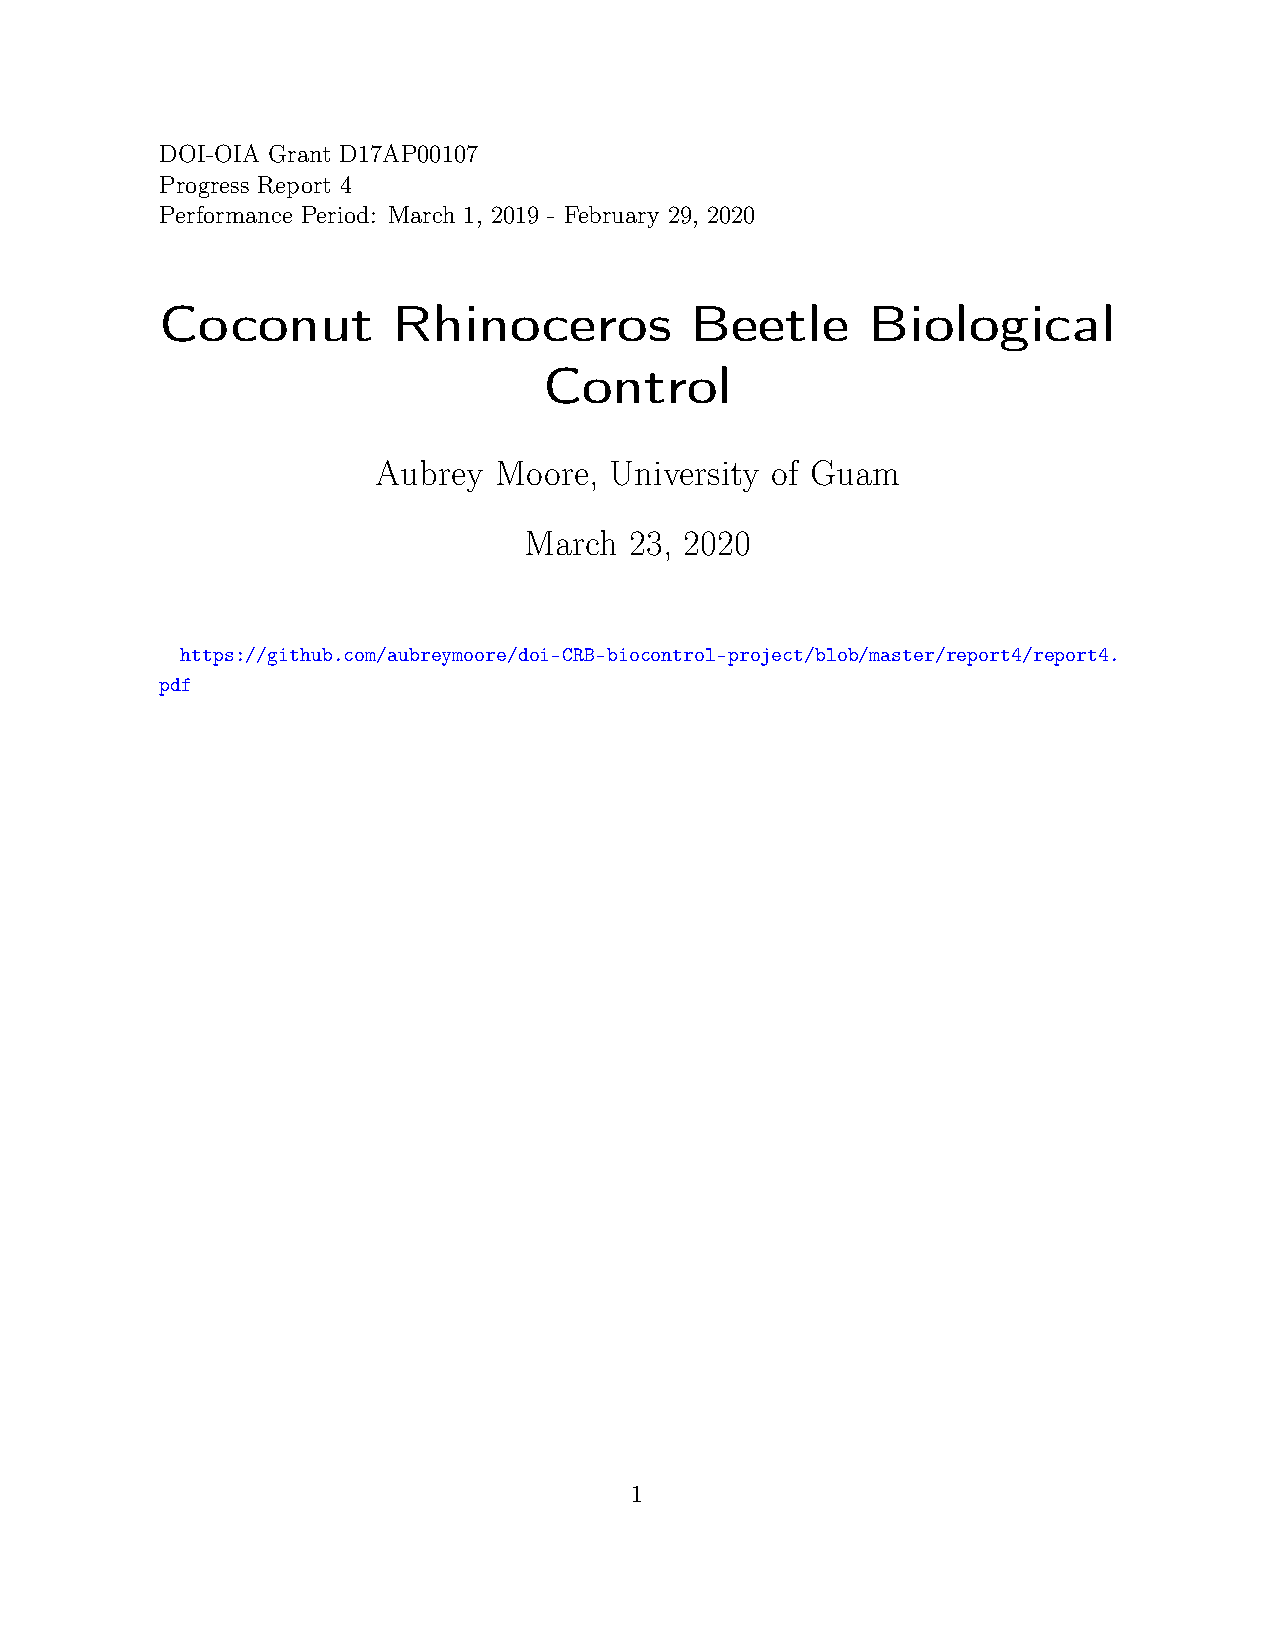
\includepdf[pages=-]{report4/report4.pdf}

%\section{\label{sec:Work-Plan-for}Work Plan for CRB-G Biocontrol Project
%Funded by USDA-APHIS}
%\includepdf[pages=-]{\string"FY17-GU-FB-CRB biocontrol workplan\string"}

\section{\label{sec:Extracts-from-the}Extracts from the 22nd Micronesian
Islands Forum Joint Communique}
\includepdf[pages=-]{\string"extracts from MF Joint Communique\string"}

\section{Letters of Support}

\subsection{Guam Legislature}
To be included when received.

\subsection{Guam Invasive Species Council}
To be included  when received.

\subsection{Micronesia Regional Invasive Species Council}
%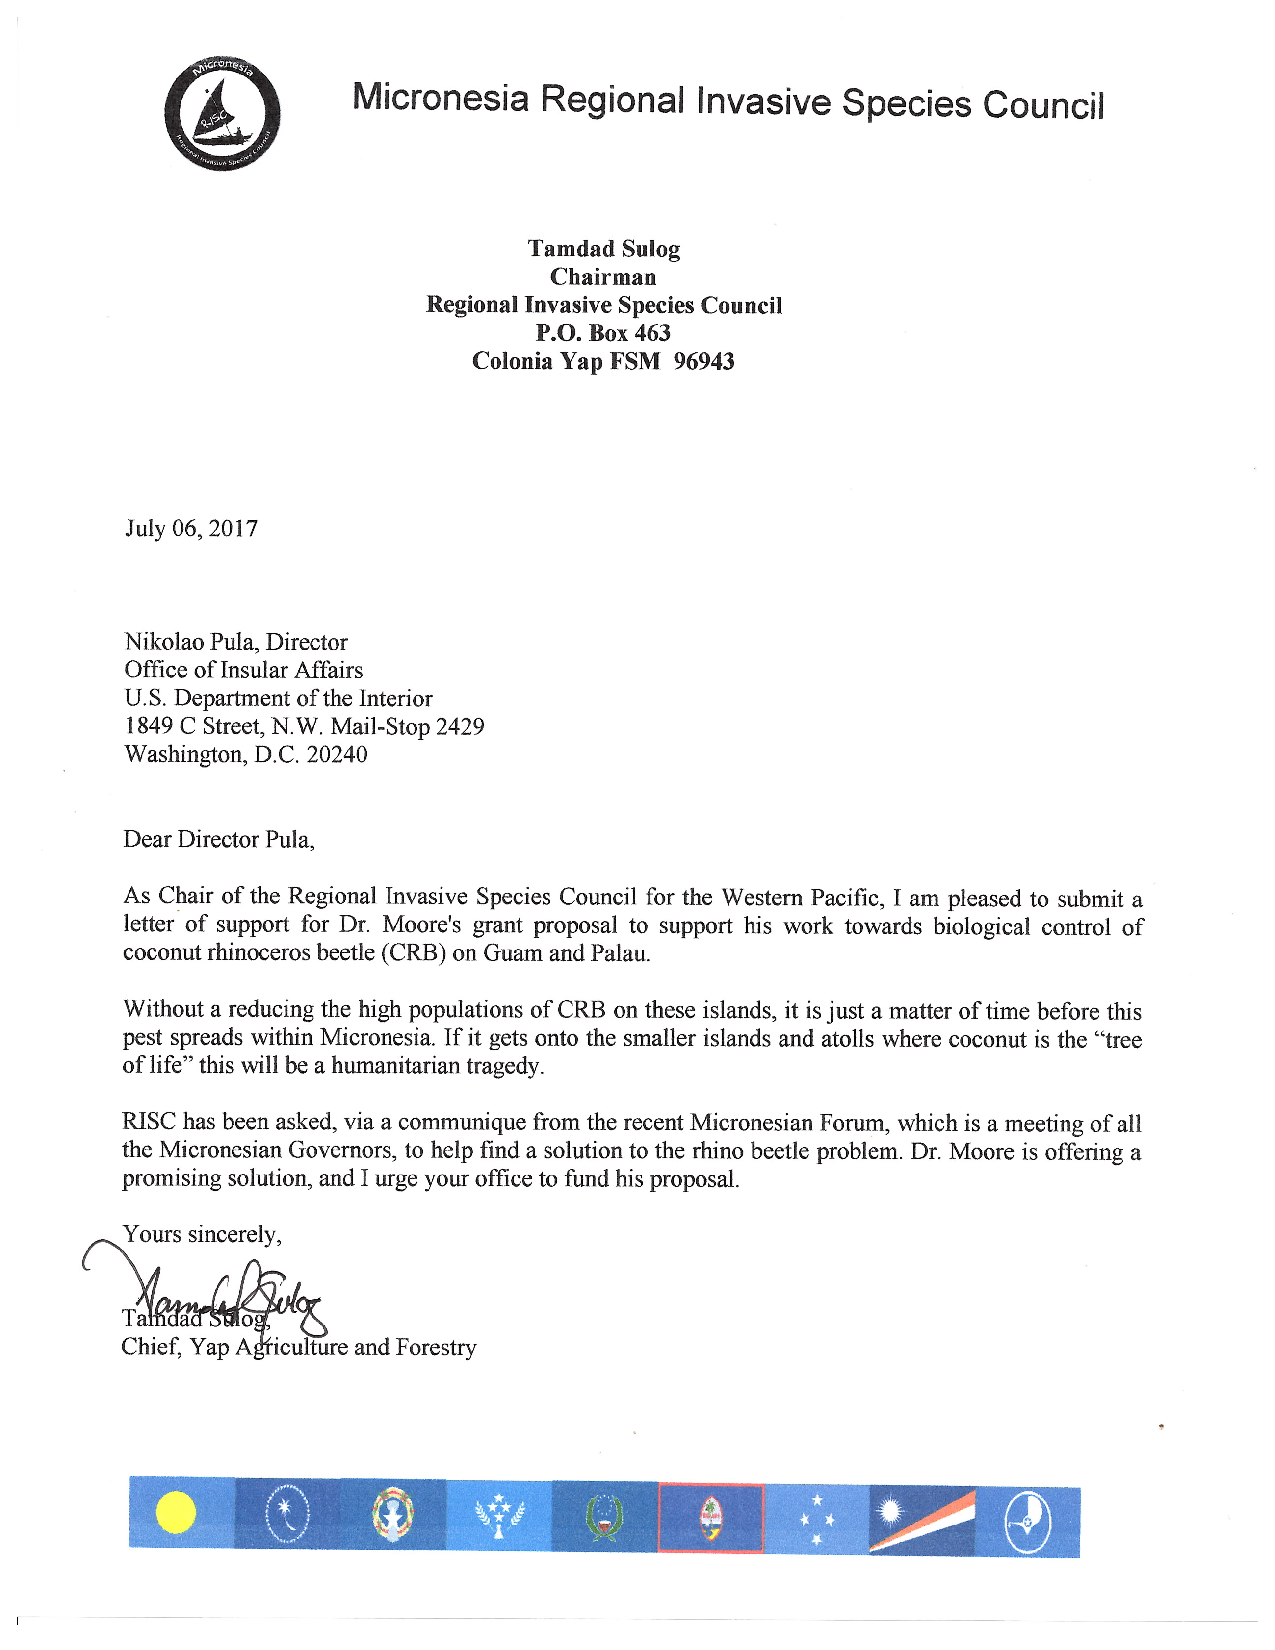
\includepdf[pages=-]{support_letters/RISC.PDF}
To be included  when received.

%\section{Administrative Forms}
%
%\subsection{SF-424}
%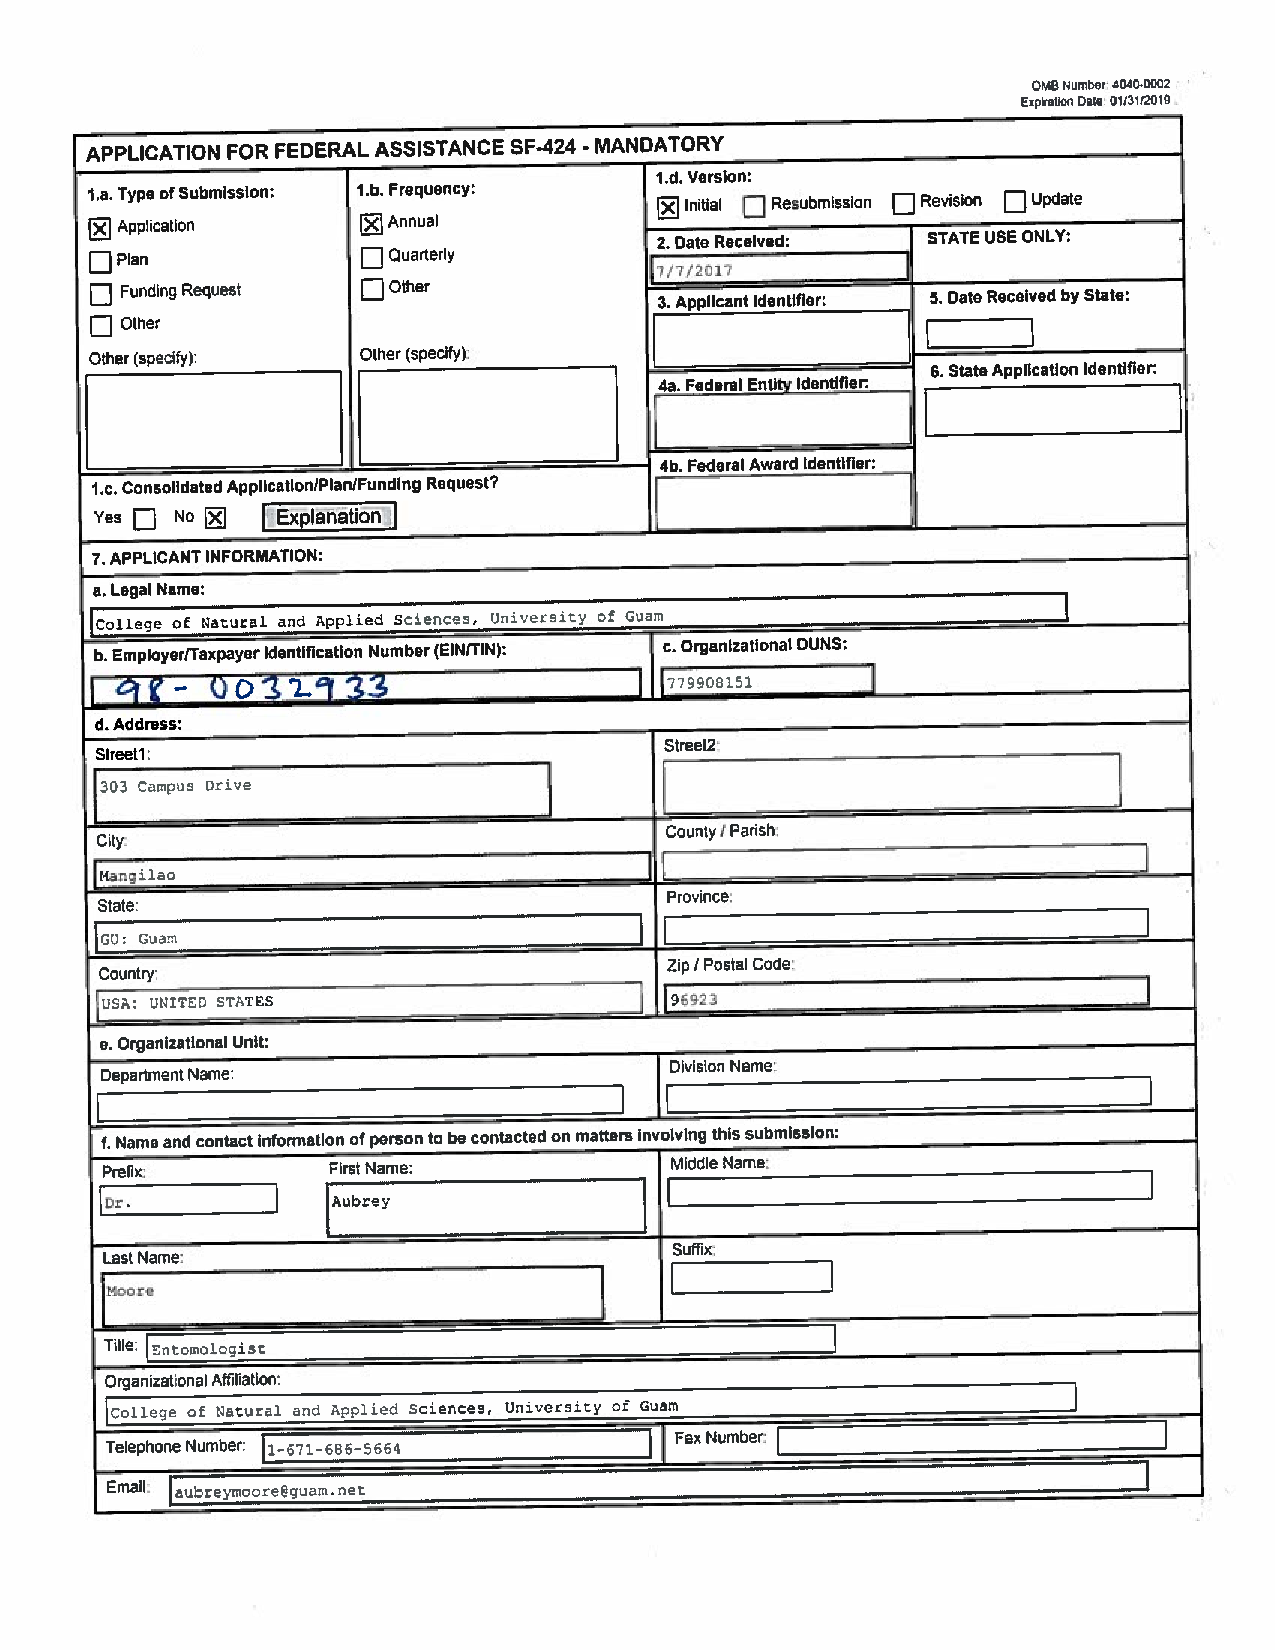
\includepdf[pages=-]{SF424_signed/SF424}
%
%\subsection{SF-424A}
%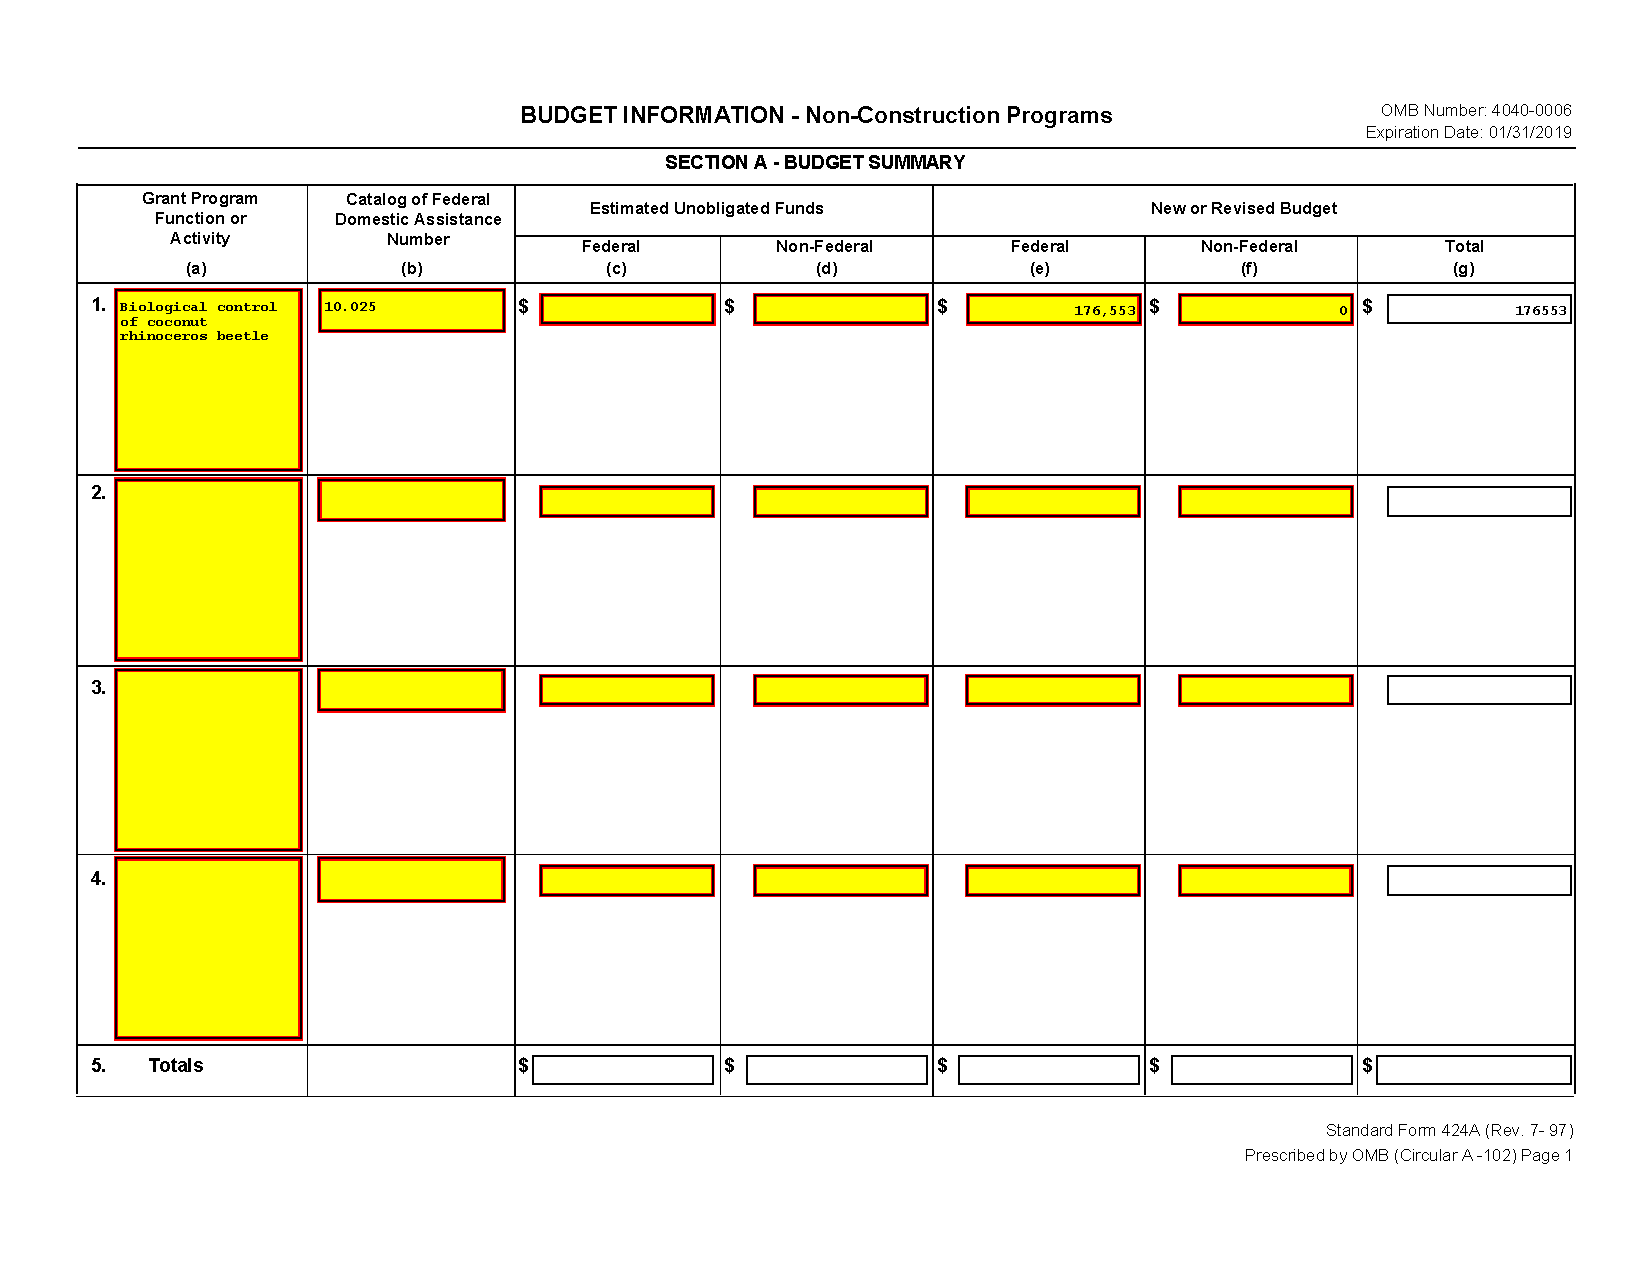
\includepdf[pages=-]{SF424_signed/SF424A}
%
%\subsection{SF-424B}
%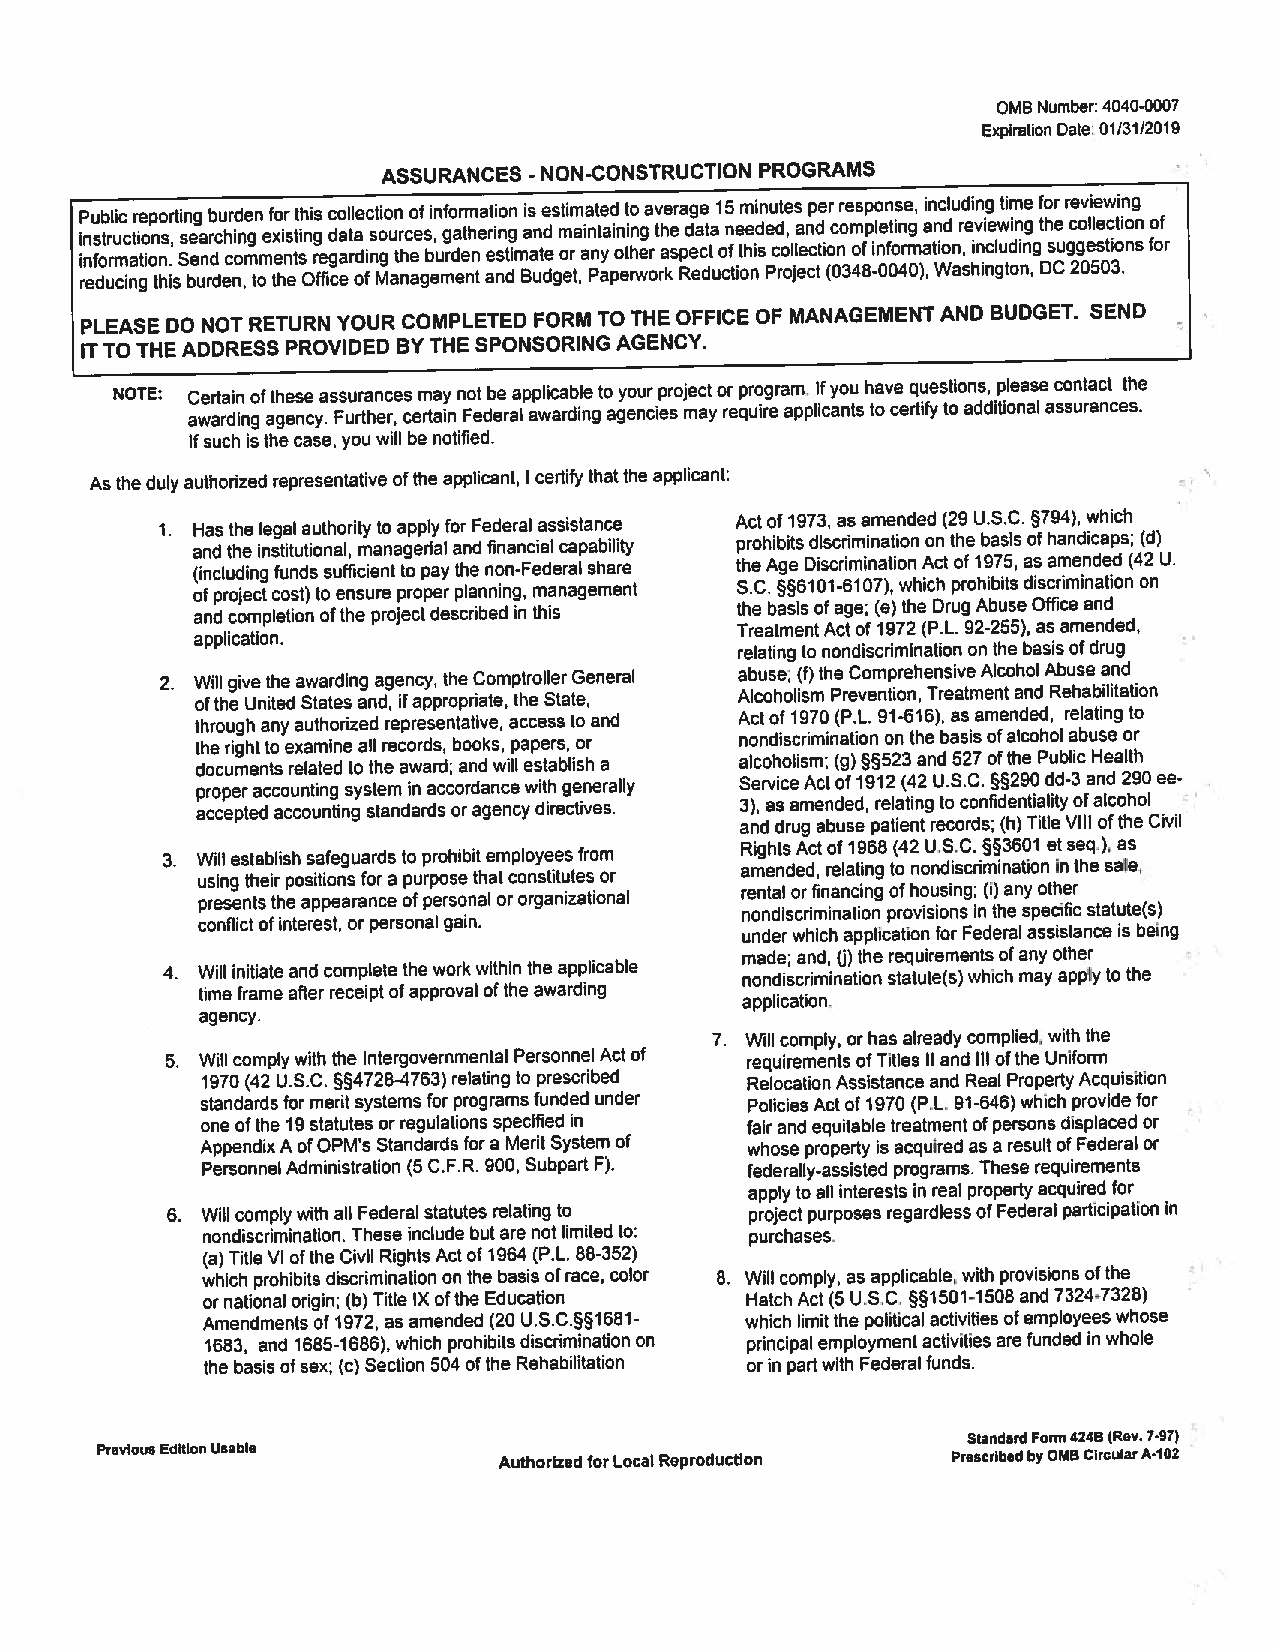
\includepdf[pages=-]{SF424_signed/SF424B}

\end{appendices}

\end{document}
